\documentclass[border=2mm]{standalone}

\usepackage{tikz}
\usepackage[american,smartlabels,fulldiodes,siunitx]{circuitikz}
\usetikzlibrary{calc}
\usetikzlibrary{shadows}
\usetikzlibrary{arrows.meta}

\usepackage{helvet}
\renewcommand{\familydefault}{\sfdefault}

\ctikzset{bipoles/thickness=1}
\ctikzset{bipoles/length=0.8cm}
\ctikzset{bipoles/diode/height=.375}
\ctikzset{bipoles/diode/width=.3}
\tikzstyle{every node}=[font=\small]
\tikzstyle{every path}=[line width=0.8pt,line cap=round,line join=round]

\newcommand{\fault}[2]{\draw[arrow,red] ($#1!0.4!#2$) to[short] +(0.05,0) -- ($#2+(-0.05,0)$);
	\draw[red] ($#1!0.4!#2$) to[short] +(-0.05,0) to[short] #1;}

\begin{document}
	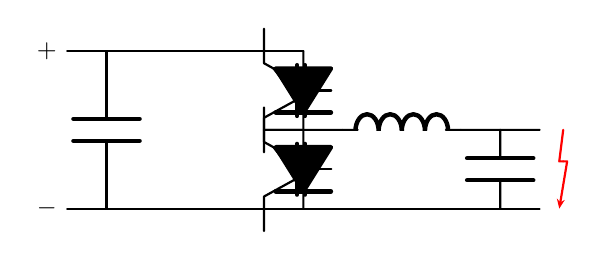
\begin{tikzpicture}
		\tikzstyle{arrow} = [-{Stealth[length=1.2mm, width=1mm]}]
		
		\coordinate (top) at (2,2);
		\coordinate (mid) at (2,1);
		\coordinate (bot) at (2,0);
		
		\draw (top) to[Tnigbt,n=S1] (mid);
		\draw (mid) to[Tnigbt,n=S2] (bot);
		
		\draw (2.5,2) to[D] (2.5,1);
		\draw (2.5,1) to[D] (2.5,0);
		\draw (top) to[short] (2.5,2);
		\draw (mid) to[short] (2.5,1);
		\draw (bot) to[short] (2.5,0);
		
		\draw (0,2) to[short] (top);
		\draw (0,0) to[short] (bot);
		\draw (0,0) to[C] (0,2);
		
		\draw (mid) to[short] (3,1);
		\draw (3,1) to[L] (4.5,1);
		\draw (4.5,1) to[short] (5,1);
		\draw (bot) to[short] (5,0);
		\draw (5,0) to[C] (5,1);
		
		\draw (5,1) to[short] (5.5,1);
		\draw (5,0) to[short] (5.5,0);
		
		\fault{($(5.5,1)+(0.3,0)$)}{($(5.5,0)+(0.3,0)$)}
		
		\draw (-0.5,2) to[short] (0,2);
		\draw (-0.5,0) to[short] (0,0);
		
		\node[anchor=east] at (-0.5,2) {$+$};
		\node[anchor=east] at (-0.5,0) {$-$};
		
	\end{tikzpicture}
\end{document}
